%%%%%%%%%%%%%%%%%%%%%%%%%%%%%%%%%%%%%%%%%%%%%%%%%%%%%%%%%%%%%%%%%%%%%%%%%%%
% filename    : sp.tex
% author      : Karl Frederick Roldan, Gerd Lowell Jana, John Kenneth Lesaba
%%%%%%%%%%%%%%%%%%%%%%%%%%%%%%%%%%%%%%%%%%%%%%%%%%%%%%%%%%%%%%%%%%%%%%%%%%%

% BUGFIX: Save LaTeX kernel version of \@xfloat
\makeatletter
\let\my@xfloat\@xfloat
\makeatother

% use ateneo de naga etd class (actually modified virginia tech's etd class)
\documentclass[oneside]{etd}

% BUGFIX: Create a modified copy of \@xfloat using the kernel definition
\makeatletter
\def\@xfloat#1[#2]{
	\my@xfloat#1[#2]%
	\def\baselinestretch{1}%
	\@normalsize \normalsize
}
\makeatother

% use these packages

\usepackage{graphicx}
\usepackage{amssymb}
\usepackage{gensymb}
\usepackage{latexsym}
\usepackage{amsmath}
%\usepackage[lineno5,noindent]{lgrind}
%\usepackage{rotating} 
%\usepackage{makeidx}
%\usepackage{stmaryrd}
\usepackage{float}
\usepackage{subfigure}
%\usepackage{cite}
%\usepackage{moreverb}
%\usepackage{pictexwd,dcpic}
\usepackage{algorithm,algorithmic}
\renewcommand{\algorithmicrequire}{\textbf{Input:}}
\renewcommand{\algorithmicensure}{\textbf{Output:}}
\usepackage{tikz}
\usetikzlibrary{positioning,calc}

\usepackage{listings}
\definecolor{cppred}{rgb}{0.6,0,0} % for strings
\definecolor{cppgreen}{rgb}{0.25,0.5,0.35} % comments
\definecolor{cpppurple}{rgb}{0.5,0,0.35} % keywords
\definecolor{cppdocblue}{rgb}{0.25,0.35,0.75} % doc
 
\lstset{language=C++,
basicstyle=\linespread{0.8}\ttfamily\small,
keywordstyle=\color{cpppurple}\bfseries,
stringstyle=\color{cppred},
commentstyle=\color{cppgreen},
morecomment=[s][\color{cppdocblue}]{/**}{*/},
numbers=left,
numberstyle=\tiny\color{black},
% stepnumber=2,
numbersep=10pt,
tabsize=4,
showspaces=false,
showstringspaces=false}

\graphicspath{{figures/}{./}}

%\renewcommand{\floatpagefraction}{0.8}

\makeindex

%%%%%%%%%%%%%%%%%%%%%%%%%%%%%%%%%%%%%%%%%%%%%%%%%%%%%%%%%%%%%%%%%%%%%%%%%%%

\title{Multiclass classification via Transformer Networks for Task Constraint-based Introductory Programming Feedback}
\author{My Name}
\department{Computer Science}
\BSdegree
\field{Computer Science}
\degreemonth{May}  % date of final defense
\degreeyear{2022}

\threestudents
{Gerd Lowell Jana}
{John Kenneth Lesaba}
{Karl Frederick Roldan}

\threestudentsheader
{Jana, Lesaba, and Roldan}

\threedegrees
{Computer Science}
{Computer Science}
{Computer Science}


\advisor
{Joshua C. Martinez, MIT}
\threemembers
{Raphael Henry M. Garay}
{Glenn G. Fabia}
{John Sixto G. Santos, MS}
\deanandchair
{Joshua C. Martinez, MIT}
{Adrian Leo Pajarillo, MS}

\keywords{CS Education, transformer}


\begin{document}

\maketitle
\makerecomm
\makeacceptance
\makedeclaration

%%%%%%%%%%%%%%%%%%%%%%%%%%%%%%%%%%%%%%%%%%%%%%%%%%%%%%%%%%%%%%%%%%%%%%%%%%%
%                    ABSTRACT/EXECUTIVE SUMMARY                           %
%%%%%%%%%%%%%%%%%%%%%%%%%%%%%%%%%%%%%%%%%%%%%%%%%%%%%%%%%%%%%%%%%%%%%%%%%%%
%execsummary
\begin{abstract}
	Task constraint feedback is a kind of feedback that checks whether problem-defined 
	constraints were fulfilled by students upon submission of work. The feedback process 
	can be as simple as checking if a certain programming construct exists or if the 
	student used a specific algorithm or data structure as prescribed by the problem. 
	Most task constraint systems, such as \textit{WeBWoRK-JAG} and \textit{Fischer06}, use basic static 
	analysis and comprehensive automated testing. ProPL, a task constraint checker, is 
	an exemption which uses natural language processing techniques to generate feedback. 
	In this study, the proponents will use Transformer Networks which have been known to 
	work really well with sequence-to-sequence natural language models such as neural 
	translation, text generation, and summarization. Previous works showed evidence 
	that transformer networks can be generalized for use in programming language processing 
	such as code generation. The study will apply transformer networks to generate classes 
	that are used in the submitted codes of students to generate relevant task constraint 
	feedback. This study aims to show how transformers can be applied in aiding computer 
	science education through task-constraint feedback.
\end{abstract}

	
\begin{dedication}

I dedicate this research work to all of humanity.

\end{dedication}


\begin{acknowledgements}

I thank everyone who helped me finish this thesis.

\end{acknowledgements}


\begingroup
\renewcommand*{\addvspace}[1]{}
\tableofcontents
% \listoffigures
% \listoftables
\endgroup

\beginbody
\pagenumbering{arabic}

%%%%%%%%%%%%%%%%%%%%%%%%%%%%%%%%%%%%%%%%%%%%%%%%%%%%%%%%%%%%%%%%%%%%%%%%%%%
\chapter{Introduction}
%%%%%%%%%%%%%%%%%%%%%%%%%%%%%%%%%%%%%%%%%%%%%%%%%%%%%%%%%%%%%%%%%%%%%%%%%%%


In the area of Information Technologies, there is a constant demand for Computer Programming. 
The application and study of fundamental concepts such as data structures and algorithms are 
needed for programmers as a core. Since competitive programming is one of the main ways to 
introduce these concepts, the assessments of these programs enable the skills of a programmer 
to develop\cite{oqvist2018coding}.

Automated assessment of programming codes has been widely used in competitive programming 
sites such as HackerEarth, CodeChef, etc.\ to aid in evaluating solutions to problem sets. 
Most of these systems utilize black-box testing wherein it inputs test cases to the submitted 
solution and compares its output to the expected output encoded by the problem setter. 
In this paper, we aim to build on existing automated program evaluation methods by adding 
algorithm detection in order to allow problem setters to fine-tune their problems by means of 
assigning and implementing task-constraints, and in turn provide a more formative feedback to 
students. The researchers will use the current state of the art Transformer Network to act as 
a classifier. This feedback system will then be implemented on Project CodeC (Coder’s Circle), 
a multifunctional web-based platform that aims to combine competitive programming, social networks, 
and a classroom-based Virtual Learning Environment (VLE), and is currently under the development 
of Ateneo de Naga University, College of Computer Studies.




\section{Project Context}

In task-constraint based feedback, an additional verification of student submission is done 
on the submission checker whether the student was able to complete the task. On a control 
structure level, this is easy since the task-constraint can be observed statically using a 
parser and checking whether the code uses an `if' or a `while', etc.

This problem is more difficult when the task is to use a certain algorithm. For example, 
a teacher may require the students to use the quicksort algorithm in the problem instead 
of mergesort. However, when a student submits a code to an automated checker, whether 
quicksort or mergesort will be unknown to the compiler due to the similar time complexities 
and may still pass the problem time and space constraints. 

Project CodeC aims to implement a task-constraint feedback system that fails a submission 
if the submitter hasn’t been able to complete the task set by the problem setter despite 
passing the space and time constraints of the problem. A sample feedback might be along the 
lines of “Oops! Are you sure you have implemented a hashmap?”


\section{Purpose and Description}
Aside from checking the submitted program’s correctness using traditional code-checking, 
Project CodeC aims to give automated formative feedback to ensure that students are 
learning through programming. One of these feedbacks is the task-constraint feedback. 
A problem setter may lay out some task requirements for the problem, such as whether to 
implement and use that specific requirement, which is useful in introductory computer 
science education.

The researchers propose the use of algorithm classification on checking whether task-requirements 
are fulfilled during the code submission. To do this, the problem setter denotes some task 
constraints which could be specific algorithms that he/she wants implemented in the student 
solution. When a student passes all the time and space constraints of the submission, the submission 
is then checked if it contains all task requirements that the problem setter had chosen. 
The feedback part notes the tasks required but were not implemented and tells the student 
that they have not implemented the said tasks. 

In this paper, we will answer the following research questions:\\
\textbf{RQ1.} How effective would the CodeBERT Transformer model be in an algorithm classification task?\\

\textbf{RQ2.} What kind of coding styles/snippets/algorithms does the Transformer perform best/worst on?

The researchers believe that no research on algorithm classification has been done yet.

\section{Objectives}
General Objective
\begin{itemize}
    \item This research aims to develop an algorithm classification machine learning model. 
\end{itemize}

Specific Objectives
\begin{itemize}
    \item A multiclass classification algorithm should be able to classify algorithms given code snippets. These code snippets will be mined from GitHub repositories containing implementations of different algorithms.
    \item The researchers will conduct studies on how the model will perform as a task-constraint feedback system using the CodeChef code submissions dataset.
    \item Also, the researchers aim to deploy the machine learning model to Project CodeC as a service if it is deemed as accurate enough for real-world use.
\end{itemize}




% \vfill\eject
\section{Scope and Limitations}

Due to the limitations on covered programming languages by CodeBERT, only Java, Python, 
and JavaScript programs will be considered. Specialized algorithms such as probabilistic 
algorithms for the traveling salesman problem and machine learning algorithms will not be 
considered. The researchers denote that an algorithm is introductory if it is covered in 
the non-Advanced chapters of introductory programming textbooks\cite{velivckovic2021clrs}\cite{skiena2020algorithm}\cite{sedgewick2011algorithms}. 

Also, since the research only covers the classification of algorithms. It does not aim to find 
if an algorithm is implemented using recursion or a for loop as that can be done using static 
analysis as shown in Chapter 2. Another area not discussed in this paper will be the effectiveness 
of task-constraint feedback systems in programming assignments for computer science education.  

%%%%%%%%%%%%%%%%%%%%%%%%%%%%%%%%%%%%%%%%%%%%%%%%%%%%%%%%%%%%%%%%%%%%%%%%%%%
\chapter{Review of Related Literature}
%%%%%%%%%%%%%%%%%%%%%%%%%%%%%%%%%%%%%%%%%%%%%%%%%%%%%%%%%%%%%%%%%%%%%%%%%%%

Competitive Programming (CP) is a sport that involves programmers competing 
against each other to solve programming problems with a time limit. The programmers 
are then evaluated based on the factors such as efficiency, time complexity, 
and the accuracy of the code.\cite{majumdar2017macacm} This paradigm was based on an 
event in Bulgaria 30 years ago called the International Olympiad in Information (IOI). 
Nowadays, the majority of these competitions are done entirely online using platforms 
such as CodeChef, HackerRank, HackerEarth, and others. It can have contestants ranging 
from two to several thousand and span topics such as data structures \& algorithms, data science, and discrete mathematics\cite{nair2020increasing}.

\section{Competitive Programming as Pedagogy}

The National University of Singapore, University of West Indies, 
and other universities have been using CP as an alternative method 
of teaching students by utilizing it as a module in replacement to intermediate-level data structures and algorithms subjects\cite{coore2019facilitating}. 
Training programs\cite{di2018learning} and teaching frameworks\cite{di2018framework} 
were also created revolving around CP as the major learning material which uses Association 
for Computing Machinery International Collegiate Programming Contest (ACM-ICPC) and IOI 
style of evaluating the performance of the students.  Furthermore, employers and graduates 
are utilizing CP as a preparatory material to adapt to the competitive environment of the 
software industry.\cite{nair2020increasing} Nair states that in India, many people joining the IT 
workforce are unemployable and use CP to increase employability and  introducing CP not 
only improves the skills of these students but also dramatically enhances their capability  of collaboration and creativity.

\section{Evaluation of Programming Codes}

Most competitive programming sites today use automatic 
assessment of programming codes that has two primary 
approaches\cite{gupta2017assessment}: Static analysis, which 
is done by inspecting the source code of the program without 
executing it; and Dynamic analysis, wherein a program is run and tested against different test cases.

\subsection{Existing methods of automated evaluation of programming codes}

Competitive programming web applications use numerous methods\cite{gupta2017assessment}\cite{nemeth2018grading} 
in evaluating programming code. Two methods have been proposed\cite{nemeth2018grading} to evaluate codes: 
\begin{enumerate}
    \item The Association for Computing Machinery (ACM) - style implements black-box testing then 
    identifies the runtime complexity and checks if it meets the maximum runtime and memory limits 
    set by the problem setter. Only the solutions that meet these requirements are given credits and the 
    most runtime efficient of them are ranked the highest. This method is used in ACM ICPC, CodeChef Cook - off contest, etc.; and 
    \item The International Olympiad in Informatics (IOI) - style evaluation first groups the test files
     according to its asymptotic complexity (e.g. $O(n)$, $O(n\log{}n)$, etc.) or logical 
     complexity(e.g. problem restricted to an easier subproblem) and are given point equivalents. 
     The judge gives the partial points to solutions that have the perfect (equal) complexity as 
     it is tested among the grouped test cases. This method is used by IOI, CodeChef Lunchtime, etc.
\end{enumerate}

Furthermore, numerous techniques\cite{haldeman2021csf}\cite{watanobe2020next}\cite{lu2018modeling}\cite{yoshizawa2019logic} were proposed in assessing programs that may further the progress in computing education.

\subsection{Task-constrained feedback in automated assessment systems}

Task-constraint feedback systems are programs that automatically give feedback on whether the 
submitted solution implements the required task. Among these systems include 
WeBWork\cite{gotel2008teaching} 
which focuses on error correction, INCOM\cite{le2009evaluation} which acts as a homework assistance system. 
The feedback from these systems are considered essential, especially in developing countries where resources 
and student-professor contact hours are limited.

Automated assessment systems perform tests that mimic that of the Software Quality Assurance (SQA) 
testing\cite{gotel2008teaching}. These tests are 
done for validation that the program does what it is intended to do, and for verification that the 
program works correctly through black-box testing. Gotel et al.\ proposed a framework that incorporates 
these SQA principles in assessing programming code. ProPL\cite{lane2005teaching} introduced a similar 
approach in identifying program goals and schemas, as well as in implementing correct solutions to problems.

\section{Sequence Models}

Sequence models are machine learning algorithms that are designed to input and/or 
output sequential data such as time series, audio, signals, texts, and videos. 
Four common sequence model types have been proposed: one-to-many, many-to-one, 
many-to-many with equal input and output lengths, and many-to-many with varying 
input and output lengths. Such models were used in applications including translation, 
image captioning, sentiment analysis, and many more\cite{yousuf2021systematic}. 

Different neural networks had been proposed with varying performance on different 
tasks in the past decades. The Recurrent Neural Network\cite{hinton1986learning} was one of 
the first sequence models that was introduced. The LSTM\cite{hochreiter1997long} 
and the GRU\cite{chung2014empirical} were introduced as modified versions of the hidden layer 
of RNN which showed significant performance improvements and eliminated the vanishing 
gradient problem of the RNN.\@ Vaswani et al.\cite{vaswani2017attention} had taken a different 
approach by introducing a model, the transformer, that takes a sequence as a whole 
instead of sequentially (as in the RNN and its variants) which renders NLP to be 
easily parallelized and self-attention which computes how words in a sequence are 
related to each other.

\subsection{Advances on Programing Language Processing in Machine Learning}

Recent breakthroughs have shown that sequence models can be generalized to 
programming languages as well. Central themes on research include code summarization\cite{xie2021exploiting} 
which can help in automatically commenting a snippet of code, 
code-clone detection\cite{wei2017supervised} which can be used for finding functional 
similarities for two code snippets that look distinct from each other, and code 
completion\cite{alon2020structural} which can be used for assistance when coding.

Processing programming languages on a neural network implies that code has 
to be embedded to a series of vectors that represent code semantics or 
syntax which can serve as input by the network. Due to this, much work 
has been done on developing ways to generate code embeddings such as 
processing Abstract Syntax Trees (AST) on CNNs and RNNs,\cite{mou2016convolutional}\cite{chen2019capturing}
descriptive program embeddings of a single code snippet on a function 
level\cite{alon2019code2vec} by encoding through AST paths\cite{alon2018code2seq}, 
and  using Hoare triples of a program\cite{piech2015learning}. 

%%%%%%%%%%%%%%%%%%%%%%%%%%%%%%%%%%%%%%%%%%%%%%%%%%%%%%%%%%%%%%%%%%%%%%%%%%%
\chapter{Theoretical Background}
%%%%%%%%%%%%%%%%%%%%%%%%%%%%%%%%%%%%%%%%%%%%%%%%%%%%%%%%%%%%%%%%%%%%%%%%%%%

\section{Transformers}

Vaswani et al\cite{vaswani2017attention} described transformers as sequence 
models that solely focus on self-attention without the need for recurrence which 
eliminates the need for unfolding during the backpropagation phase of learning. 
In the paper, attention was defined with respect to keys, values, and queries. 
The attention is computed with

\[ 
    attention(K,Q,V) = \left(\frac{QK^T}{\sqrt{dim(K)}}\right)V 
\]

where K is the key matrix, Q is the query matrix, and V is the value matrix. 
The dot product of Q and K is scaled by the square root of the dimension of K.

Transformer models take the whole input as a whole instead of recurrently meaning 
that the model does not know the order of the words in the sequence. Hence, the 
paper proposed the use of positional encodings through sinusoidal functions 
added to the embedded vectors. Suppose that W is a matrix where each column 
corresponds to a position pos and each row i corresponds to the individual 
dimensions in the model which alters the frequency. Let 
\begin{math}
    W=10000^2i/embedsize
\end{math}
where embedsize is a hyperparameter which is also the embedding size of the 
embedded vectors. Then, the positional encoding is calculated by
\[ 
    POS(pos,i) = \sin\left(\frac{pos}{W}\right) \text{if \textit{i} is even and}
\]
\[ 
    POS(pos,i) = \cos\left(\frac{pos}{W}\right) \text{if \textit{i} is odd}
\]
The key component of transformers is the multi-headed attention layer, wherein 
attention is computed multiple times and concatenated together. Transformers 
were able to outperform established models for machine translation with 
English-German translation.

\section{RoBERTa for Classification}
RoBERTa\cite{liu2019roberta} is a replication study of the original BERT 
model by finer-tuning hyperparameters and removing the Next Sentence 
Prediction task which was shown that it does not negatively affect the 
performance of the model. While the original transformer by Vaswani et al.\ 
is a Seq2Seq transformer, RoBERTa is an autoencoder transformer trained on a 
large corpus, which can be used with fine-tuning or transfer learning for 
different downstream tasks such as classification\cite{pritzkau2021nlytics}.

In this paper, the researchers will use the CodeBERT\cite{feng2020codebert} 
to be used with transfer learning on algorithm classification. The CodeBERT 
model is a variant of RoBERTa pretrained on multiple programming languages 
including Java, Python, and Javascript.

\subsection{Model Architecture}

The CodeBERT model is a bidirectional transformer using a similar architecture 
with RoBERTa without any architectural modification.

\subsection{Dataset}

CodeBERT was trained on a large corpus of about 8million codes of both bimodal 
and unimodal data. Bimodal data means that for each code snippet, 
there is an accompanying natural language snippet while unimodal data 
implies the absence of the natural language snippet. The data were gathered from 
GitHub, which was collected by Husain et al\cite{husain2020codesearchnet}.

\section{Task-Constraint Feedback}

Knowledge About Task-Constraints (KTC) feedback systems employ the use of limiting 
the submission by adding requirements, called \textit{constraints}, that will tell the 
student if they haven’t completed the requirement.\cite{keuning2016towards} One of the methods used 
is \textit{Hints on Task Requirements} (TR) wherein a hint will be given when a task was 
not completed. As an example, suppose that the problem setter asked to balance a 
binary search tree using red-black trees. However, the submitter was able to 
complete the problem using an AVL tree. The TR system should give some feedback 
that the Red-Black Tree is a requirement for the given problem.

\section{Algorithm Classification}
Algorithms and data structure can be written multiple ways with different stylistic 
and data structure choices. The researchers define algorithm classification as to 
what algorithm some code snippet is implementing, rather than the class such as 
sorting, searching, etc. Introductory algorithm textbooks\cite{velivckovic2021clrs}\cite{skiena2020algorithm}\cite{sedgewick2011algorithms} 
have a good resource on the algorithm names through its table of contents which will 
be used as labels in the classifier. With this, this research defines algorithm 
classification by tagging code snippets as to the question “what is the algorithm 
name that this code snippet is implementing?” 

In computer science education, students might use multiple algorithms into one file 
and begin using different data structures for their implementations. As an example, 
consider the task of implementing a \textit{priority queue} (the \textit{priority queue} is a classification). 
The priority queue data structure can be implemented with \textit{binary heaps} or dictionaries 
such as \textit{linked lists} and \textit{binary search trees}; in this example, assume that the priority 
queue is implemented with a \textit{binary heap}. Introductory programming students might usually 
be coding these algorithms and algorithms manually into one file and it is not enough to 
say that the submission implements a \textit{priority queue} since a \textit{binary heap} is also implemented. 

Suppose that the code snippet implements an algorithm and uses some data structure or 
another algorithm using the language’s standard library, then the snippet will only be 
classified using the manual implementation disregarding the standard library function. 
Likewise, code snippets that do not belong to any algorithms stated in any of the 
introductory algorithm textbooks are said not to use any algorithm. These code snippets 
usually contain the \textit{main} function (but not always), setter and getter functions, 
and boilerplate codes.

%%%%%%%%%%%%%%%%%%%%%%%%%%%%%%%%%%%%%%%%%%%%%%%%%%%%%%%%%%%%%%%%%%%%%%%%%%%
\chapter{Methodology}
%%%%%%%%%%%%%%%%%%%%%%%%%%%%%%%%%%%%%%%%%%%%%%%%%%%%%%%%%%%%%%%%%%%%%%%%%%%



\section{Dataset}

The researchers will be using a custom dataset mined from public GitHub 
repositories that contain Python, JavaScript, and Java source code, such as 
those repositories that implement  algorithms and data structures. Labels 
will be extracted from a number of heuristics such as method name or the 
repository folder in the case of algorithm implementation datasets. Since 
CodeBERT only accepts input lengths of less than 512, it is important to 
preprocess the dataset to make sure that each code snippet contains less than 
512 tokens\cite{devlin2018bert}\cite{liu2019roberta}.

\textbf{RQ1.} Data Augmentation\cite{feng2021survey}
will be done to make the dataset synthetically larger. To counter the challenge of 
overfitting, that is, making sure that the model will not simply memorize variable 
names, the researchers will be using synonym replacements on identifiers and swapping 
consecutive lines that are declaring variables as these do not have an effect on the code. 
Custom code extraction programs will be written for each programming language using available parsers.

\textbf{RQ2.} Code snippets should be able to preserve coding styles except for the 
comments which will not be considered.

\section{Training}

CodeBERT will be used for transfer learning on the custom dataset using a multiclass 
classification task with each one-hot encoded label corresponding to one algorithm. 
Different hyperparameters on the output layer will be used for model selection. The 
researchers will make use of the PyTorch\cite{paszke2019pytorch} library for implementation 
and PyTorch Lightning for training\cite{Falcon_PyTorch_Lightning_2019}.

\section{Model Selection}

The best performing model will be selected with the criteria based on its F1-score.
Precision and recall are metrics that are calculated based on the true positives, 
false positives, true negatives, and false negatives given by the formulae. 
Once the best model has been selected, a prototype implementation of Project 
CodeC’s task-constrained feedback feature will be implemented to test on 
actual programming competition datasets. \( precision = \frac{true positive}{true positive + false positive}\) and 
\( recall = \frac{true positive}{true positive + false negative}\). The F1 score balances these metrics using the formula 
\( F1 = \frac{2(precision)(recall)}{precision + recall}\).\newline

\textbf{RQ1.} The model with the highest F1 score must be the one with the best performing model. 
Other performance metrics may be collected such as running loss and classification accuracy.

\textbf{RQ2.} By recording the examples that resulted in false positives and false negatives, manual analysis will 
be performed to identify the features that the transformer was not able to fully capture.



% %%%%%%%%%%%%%%%%%%%%%%%%%%%%%%%%%%%%%%%%%%%%%%%%%%%%%%%%%%%%%%%%%%%%%%%%%%%
\chapter{Results}
%%%%%%%%%%%%%%%%%%%%%%%%%%%%%%%%%%%%%%%%%%%%%%%%%%%%%%%%%%%%%%%%%%%%%%%%%%%


% %%%%%%%%%%%%%%%%%%%%%%%%%%%%%%%%%%%%%%%%%%%%%%%%%%%%%%%%%%%%%%%%%%%%%%%%%%%
\chapter{Contributions and Recommendations}
%%%%%%%%%%%%%%%%%%%%%%%%%%%%%%%%%%%%%%%%%%%%%%%%%%%%%%%%%%%%%%%%%%%%%%%%%%%

\section{Summary of Contributions}


\section{Recommendations}


There could be several reasons why our tests did not yield the ``same'' results as that of \cite{Zaritsky2004}'s.
The author claims that this may be due to the myriad of parameters used in evolving
individuals in each step of the genetic algorithm and the large number of possible candidates or values that we can set these parameters with. 
For example, we may claim that the appropriate choice of the recombination technique is necessary. In \cite{Zaritsky2004},
a two-point crossover was employed. Thinking that this may be less of a factor, the author proceeded with just
one-point cross in implementing the genetic algorithm for the experiment.
Another could be in choice of the probabilities associated with recombination, elitism, and mutation rates.
The author did only consider what was stated in the base paper without performing tests to validate
whether this values are appropriate and could still complement the change made in some of the assumptions.
As such, more empirical tests could be done to appropriately estimate these parameters. 

If indeed DNA sequence assembly is the task at hand, lots of other techniques are now available.
One may consider for example representing the reads or DNA fragments in a de Bruijn graph
as opposed to the overlap graph presented in this paper. 
Assembling reads  in a de Bruijn graph 
reduces the problem to a fragment assembly problem that can be 
formulated as the goal to find a trail or Eularian path that visits 
each edge (read or fragment) in the (de Bruijn) graph exactly once. 
Such, somehow makes the assembly process much ``easier'' since Eularian path
construction is known to be solvable in deterministic polynomial time.



\appendix
\chapter{Research Timeline}

\begin{center}
    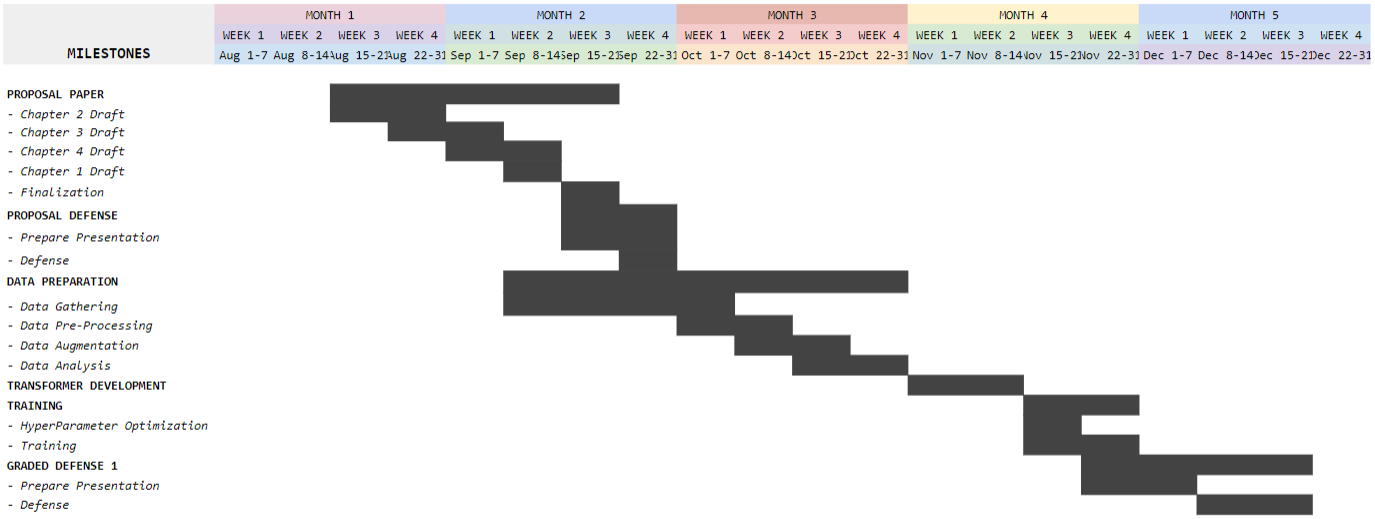
\includegraphics[width=\textwidth]{figures/first-sem.pdf}
    First Semester Timeline
\end{center}

\begin{center}
    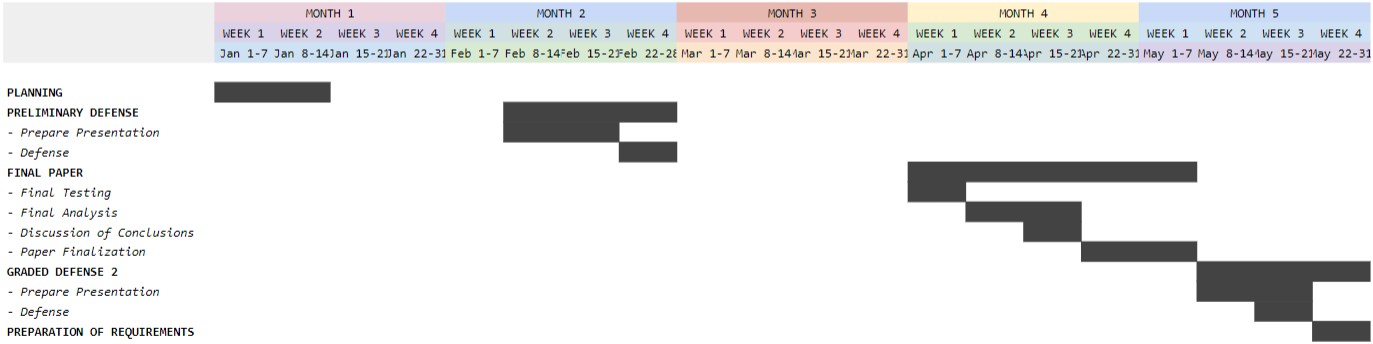
\includegraphics[width=\textwidth]{figures/second-sem.pdf}
    Second Semester Timeline
\end{center}
% \chapter{Evaluation Tool}

Evaluation tool used goes here.

% \chapter{Sample Reports}

Describe and discuss the details of sample reports here.

% \chapter{Sample Input/Output}

Describe and discuss the details of sample I/O here.

% \chapter{Code Listing}

\lstinputlisting{src/scs-greedy.cpp}

% \chapter{User's Guide}

\begin{center}
    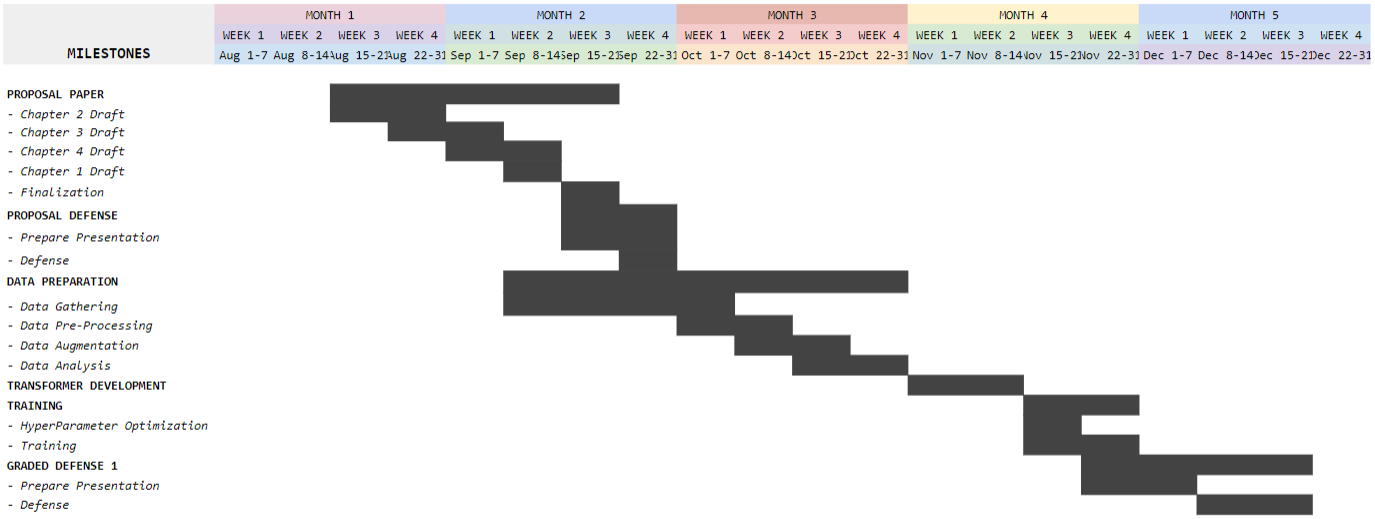
\includegraphics[width=\textwidth]{figures/first-sem.pdf}
    Figure 4.1.1 Centralized client-server architecture
\end{center}

\begin{center}
    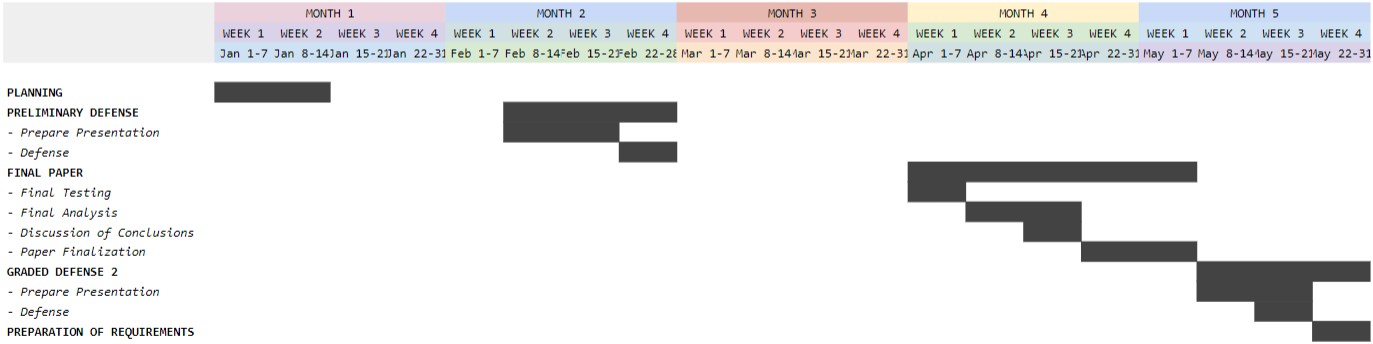
\includegraphics[width=\textwidth]{figures/second-sem.pdf}
    Figure 4.1.1 Centralized client-server architecture
\end{center}



\nocite{*}
\bibliographystyle{siam}
\bibliography{sources.bib}



% \begin{vita}
JR is BS Information Technology student of the
Department of Computer Science at the Ateneo de Naga University.
\end{vita}



\end{document}
